\section*{Задание 1}
Написать хвостовую рекурсивную функцию my-reverse, которая развернет верхний
уровень своего списка-аргумента lst.

Создать базу знаний «Собственники», дополнив (и минимально изменив) базу знаний, хранящую знания:
\begin{itemize}
	\item «Телефонный справочник»: Фамилия, Noтел, Адрес – структура (Город, Улица, Noдома, Noкв),
	\item «Автомобили»: Фамилия\_владельца, Марка, Цвет, Стоимость, и др.,
	\item «Вкладчики банков»: Фамилия, Банк, счет, сумма, др.
\end{itemize}
знаниями о дополнительной собственности владельца. Преобразовать знания об автомобиле к форме знаний о собственности. Вид собственности (кроме автомобиля):
\begin{itemize}
	\item Строение, стоимость и другие его характеристики;
	\item Участок, стоимость и другие его характеристики;
	\item Водный\_транспорт, стоимость и другие его характеристики.
\end{itemize}

Описать и использовать вариантный домен: Собственность. Владелец может иметь, но только один объект каждого вида собственности (это касается и автомобиля), или не иметь некоторых видов собственности.

Используя конъюнктивное правило и разные формы задания одного вопроса (пояснять для какого No задания – какой вопрос), обеспечить возможность поиска:
\begin{enumerate}
	\item Названий всех объектов собственности заданного субъекта,
	\item Названий и стоимости всех объектов собственности заданного субъекта,
	\item * Разработать правило, позволяющее найти суммарную стоимость всех
	объектов собственности заданного субъекта.
\end{enumerate}

Для 2-го пункт и одной фамилии составить таблицу, отражающую конкретный
порядок работы системы, с объяснениями порядка работы и особенностей использования доменов (указать конкретные Т1 и Т2 и полную подстановку на каждом шаге)

\begin{lstinputlisting}[label=third,caption=Решение задания №1, language=prolog, firstline=1, lastline=53]{../lab_13.pro}
\end{lstinputlisting}

\begin{figure}[H]
	\caption{Таблица к заданию.}
	\begin{center}
		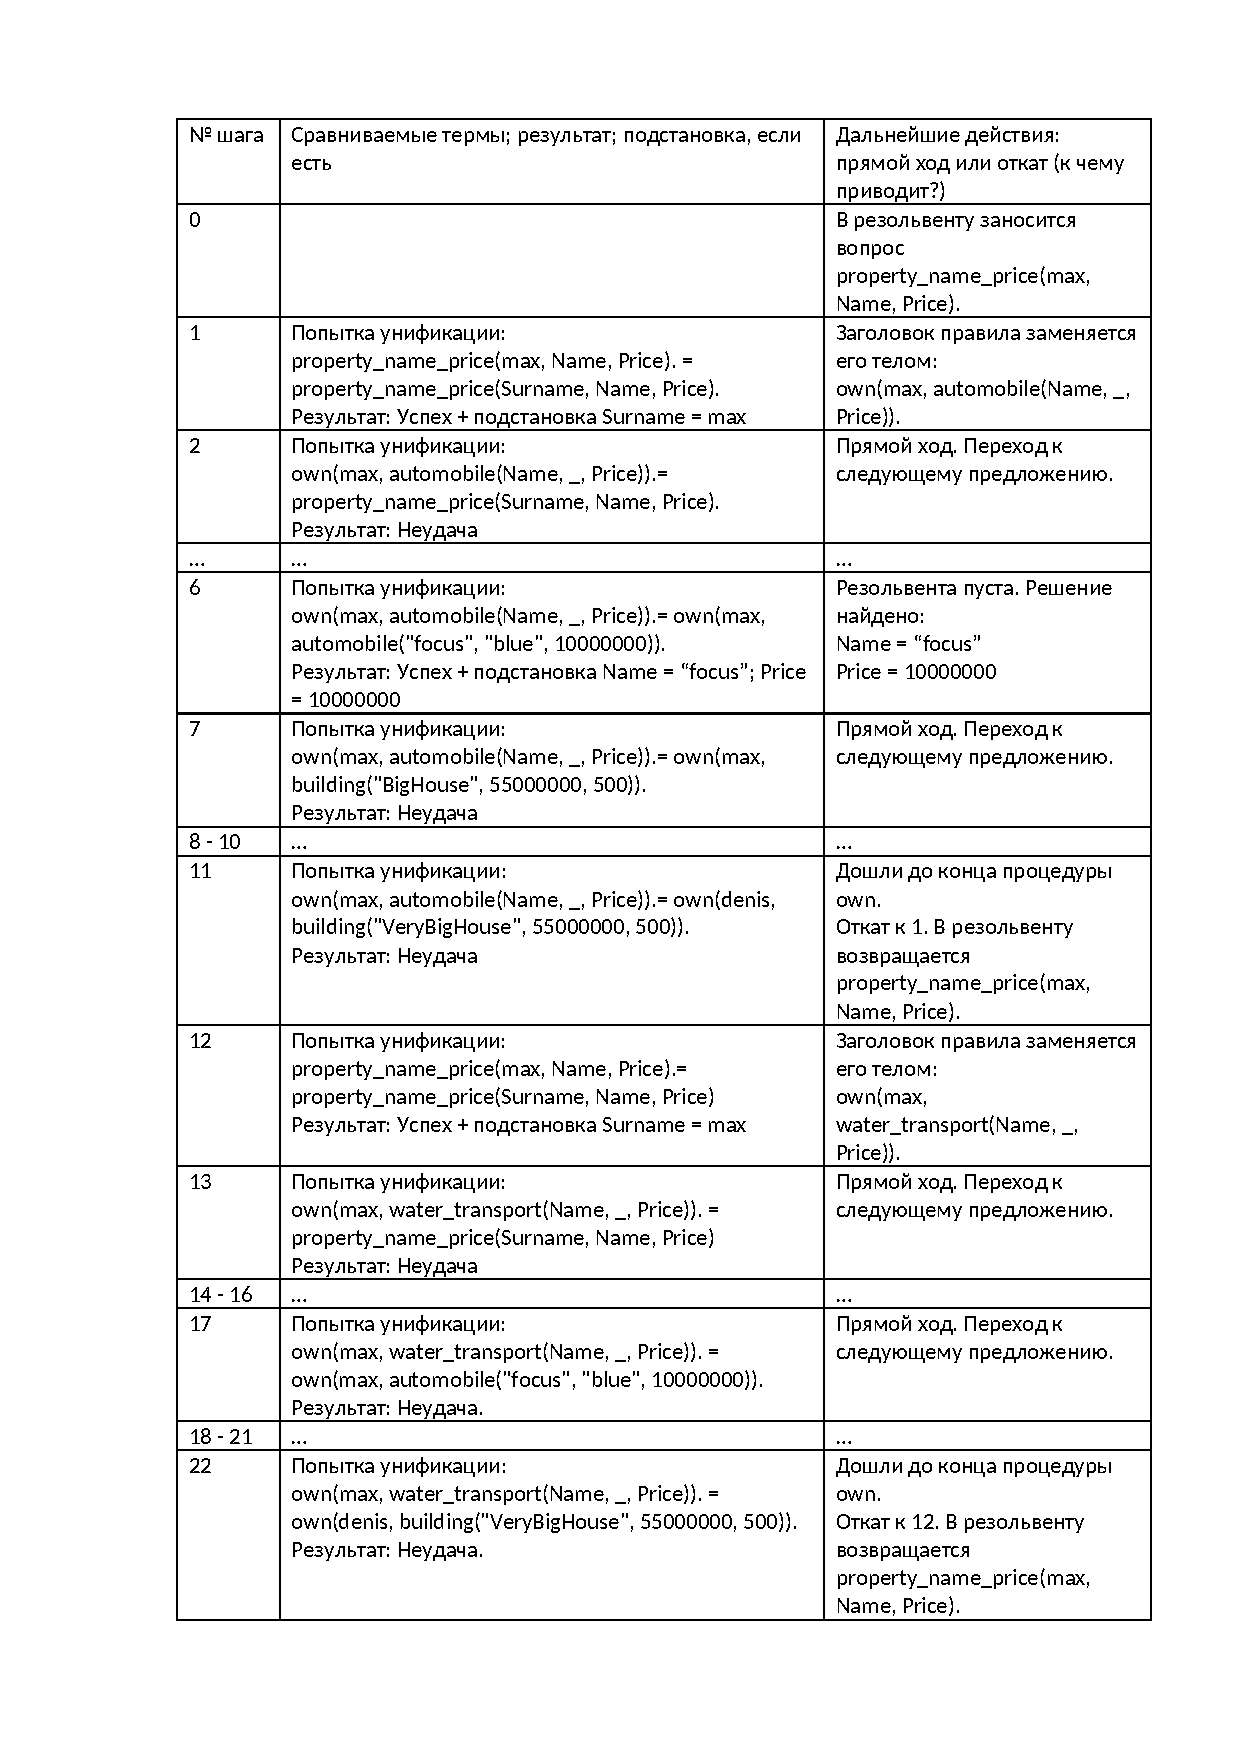
\includegraphics[scale=0.85]{img/13.1.pdf}
	\end{center}
	
\end{figure}

\begin{figure}[H]
	\begin{center}
		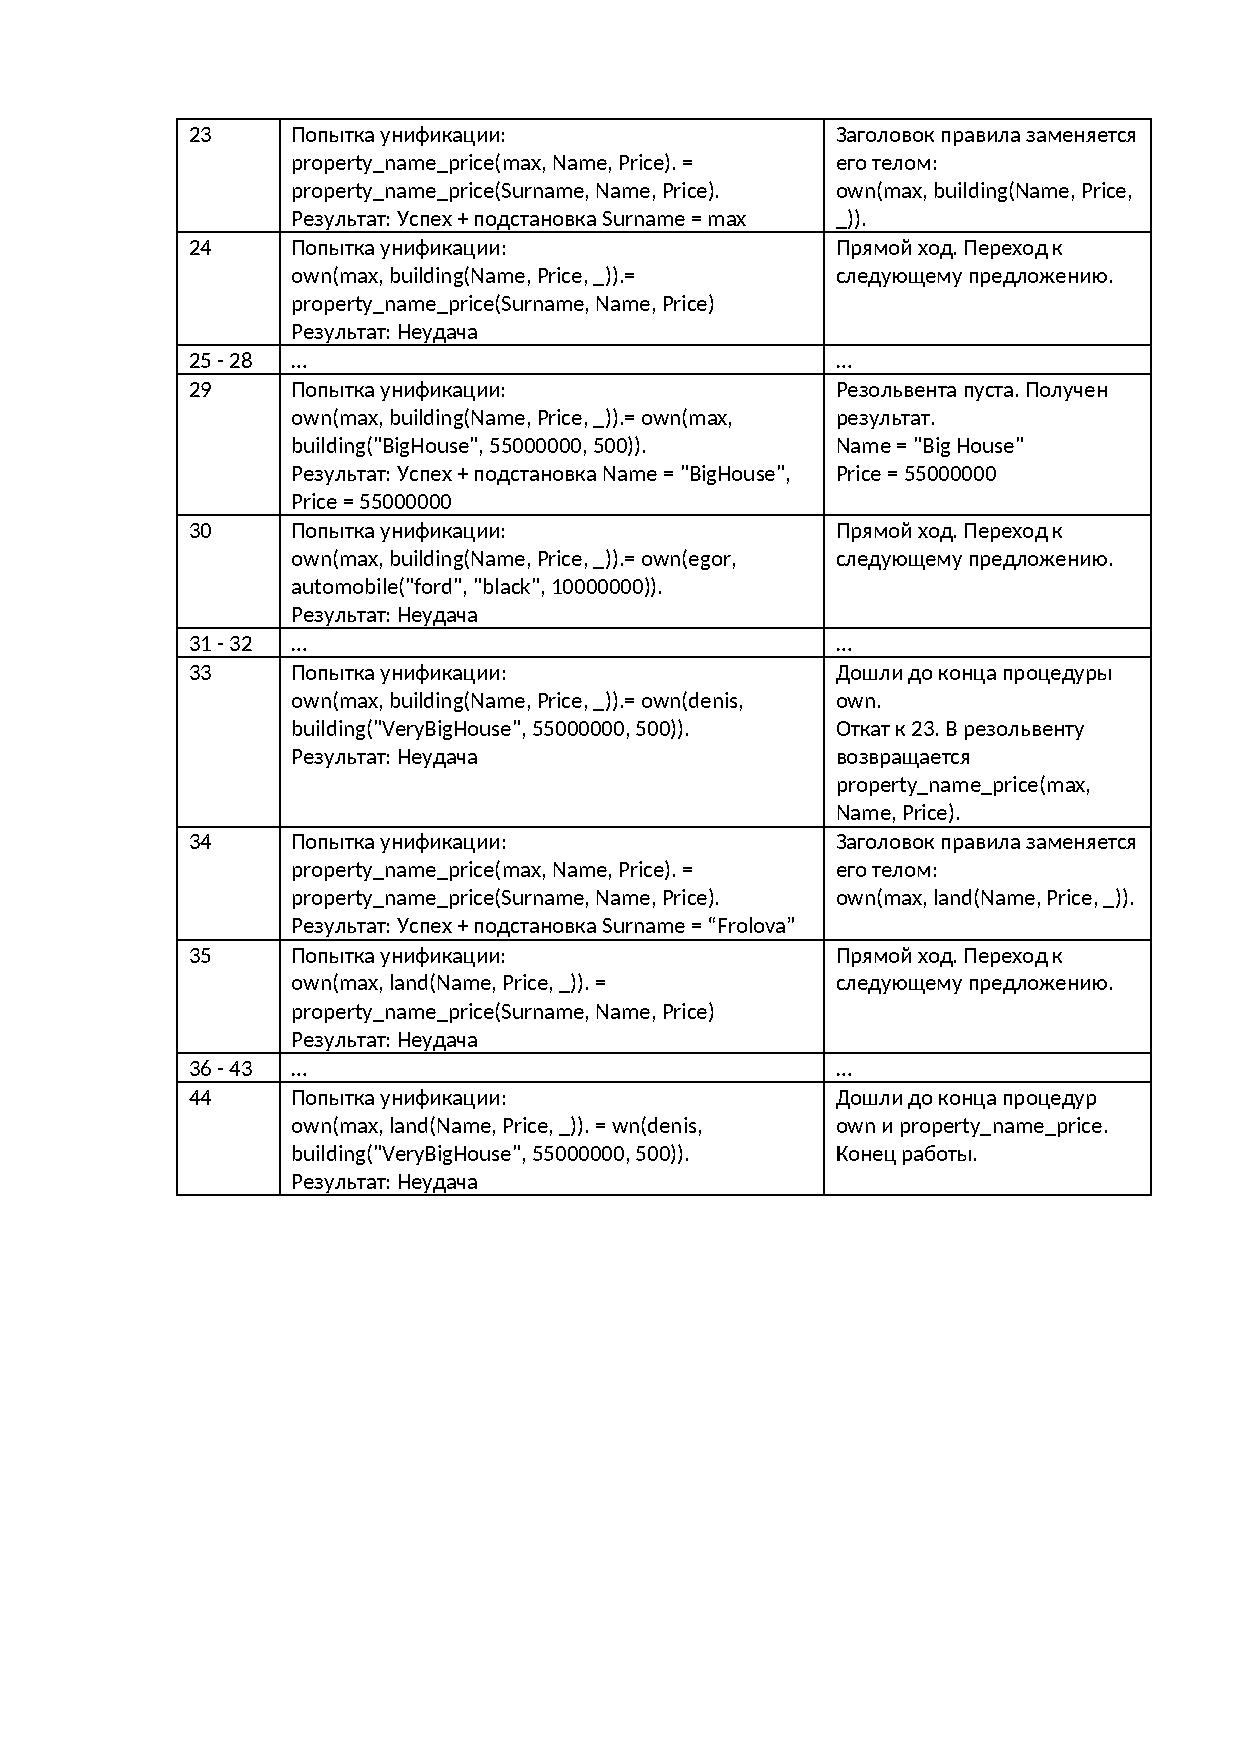
\includegraphics[scale=0.85]{img/13.2.pdf}
	\end{center}
	
\end{figure}